\begin{section}{Fisher Information Content}
  \label{sec:fisherinfo}
  Mathamatically, the Fisher information $I$ of the initial scale
  invariant matter power spectrum, $A$, is defined as
  \begin{align}
    I_A \equiv -\left\langle \frac{\partial ^2 \mathrm{ln \Largr}}{\partial  \mathrm{ln} A ^2}\right\rangle,
    \label{eq:fisherdefine}
  \end{align}
  in which $\Largr$ denotes the likelihood \cite{bib:Tegmark1997}.  
  In this paper, the word \enquote{information} and the symbol \enquote{$I$} both implicitly 
  mean cumulative Fisher information 
  of $A$. For Gaussian
  fluctuations, the likelihood depends on parameters only through the
  power spectrum $P(k)$, so $I$ can be written as 
  \begin{align}
    I = - \left\langle \sum_{k,k'} \frac{\partial \mathrm{ln} P(k)}{\partial \mathrm{ln} A} 
    \frac{\partial ^2 \mathrm{ln \Largr}}{\partial \mathrm{ln} P(k) \partial \mathrm{ln} P(k')}
    \frac{\partial \mathrm{ln} P(k')}{\partial \mathrm{ln} A}\right\rangle,
    \label{eq:fisherdef2}
  \end{align}
  in which the angle bracket denotes the average of many realizations
  of the power spectrum \cite{bib:Rimes2006}.

  Eq.~\ref{eq:fisherdef2} can be written in a simpler
  form in two aspects.   First, we can simplify the derivative terms
  $\partial \mathrm{ln} P(k)/\partial\mathrm{ln} A$.  For a given density field $\delta_a$, we can
  conveniently decompose it into linear and non-linear components
  \begin{align}
    \delta_a(k) = b (k) \delta _L (k) + \delta_{n}(k),
    \label{eq:decompose}
  \end{align}
  in which $\delta_L$ denotes the linear density field, $b(k)$ is the
  bias and $\delta_{n}(k)$ is defined such that the correlation
  $\langle \delta_L(k)\delta_{n}(k) \rangle$ is zero.  If we correlate
  $\delta_a$ and $\delta_L$,
  \begin{align}
    \langle \delta_a(k)\delta_L(k) \rangle = b(k) \langle \delta_L(k)\delta_L(k) \rangle,
    \label{eq:correlating}
  \end{align} 
  we can solve for $b$ as
  \begin{align}
    b (k) = \frac{P _{aL}(k)}{P_{LL}(k)}.
    \label{eq:bofk}
  \end{align}
  To find the non-linear term, we correlate $\delta_a$ with itself,
  \begin{align}
    \langle \delta_a(k) \delta_a(k) \rangle = 
    b^2(k) \langle \delta_L(k) \delta_L(k) \rangle + \langle \delta_{n}(k)\delta_{n}(k) \rangle,
  \end{align}
  and find
  \begin{align}
    P_{aa}(k) = b^2(k) P_{LL}(k) + P_{nn}(k).
    \label{eq:powerdecompose}
  \end{align}
  With the help of Eq.~\ref{eq:bofk} and Eq.~\ref{eq:powerdecompose},
  we get
  \begin{align}
    \frac{\partial \mathrm{ln} P(k) }{ \partial \mathrm{ln} A}=
    \frac{P_{LL}(k)}{P_{aa}(k)}b^2(k)=r^2_{aL}(k).
  \end{align}

  The second step we can make is to simplify
  $\partial ^2 \mathrm{ln \Largr}/\partial \mathrm{ln} P(k) \partial
  \mathrm{ln} P(k')$
  by utilizing the fact that its expectation value is the Fisher
  matrix.  For linear fields, this is equal to the inverse of the
  covariance matrix which is diagonal with elements given by the
  number of modes in each bin (when considering $\bs{k}$ and $-\bs{k}$ as the same mode).  
  We can extend this definition to
  non-linear fields, provided we take into account that the covariance
  matrix is no longer diagonal and invert it appropriately \cite{bib:Rimes2006}.  Thus, we
  can write the Fisher information in terms of matrix multiplication:
  \begin{align}
    I \left( < k_n\right) = r^2(k)^{\mathrm{T}} \left[ \mathrm{C^{-1}_{norm}} 
    ( k,k' )\right]_{<k_n} r^2(k') ,
    \label{eq:fisherformulaused}
  \end{align}
  where $\mathrm{C_{norm}}$ is the normalized covariance matrix
  defined as
  \begin{align}
    \mathrm{C_{norm}} \left( k,k' \right)=\frac{\mathrm{Cov}(k,k')}
    {\langle P(k)\rangle\langle P(k')\rangle},
  \end{align}
  $r$ is the mean cross correlation of a given density field with
  linear one and the subscript $<k_n$ indicates the matrix is set to
  zero for modes $k,k'>k_n$.  The elements of the covariance matrix are defined as
  \begin{align}
    \mathrm{Cov}\left(k,k'\right)\equiv \frac{\sum_{i,j=1}^{N}\left[ P_i \left( k \right) - 
    \langle P \left( k \right) \rangle \right]\left[ P_j \left( k' \right) - 
    \langle P \left( k' \right)\rangle \right]}{N-1},
  \end{align}
  where $N$ is the total number of simulations and angle brackets are
  values averaged over all simulations.  

  The cross-correlation coefficient matrix, or for short the correlation matrix, 
  is defined as :
  \begin{align}
    \mathrm{Corr}\left(k,k'\right)=\frac{\mathrm{Cov}\left(k,k'\right)}
    {\sqrt{\mathrm{Cov}\left(k,k\right)\mathrm{Cov}\left(k',k'\right)}},
  \end{align}
  and represents the correlation between different $k$ modes.  The
  corelation matrices for non-linear and reconstructed power spectra
  are shown in the upper-left and lower-right sections of Fig.~\ref{fig:corrall}.
  By definition, the correlation matrix is symmetric with unit
  diagonal allowing us to overlay the two matrices.  For the
  non-linear case, the correlation matrix is almost diagonal in the linear
  regime, $k \lesssim 0.07$ h/Mpc.  The off-diagonal
  elements are produced by strong mode coupling on non-linear scales
  and the super-survey tidal effect which is small on linear scales
  but dominates in the weakly non-linear regime
  \cite{bib:Kazuyuki2016}.  The correlation matrix for the non-linear
  power spectra has a few negative elements
  ($\mathrm{Corr} \gtrsim -0.18$), which should vanish with more
  simulations \cite{bib:Takahashi2009}.  For the reconstructed
  correlation matrix, the linear regime expands up to $k \simeq 0.3$
  h/Mpc.  However, the number and magnitude of negative off-diagonal
  elements also increases ($\mathrm{Corr} \gtrsim -0.48$).

  \begin{figure}
    \centering
    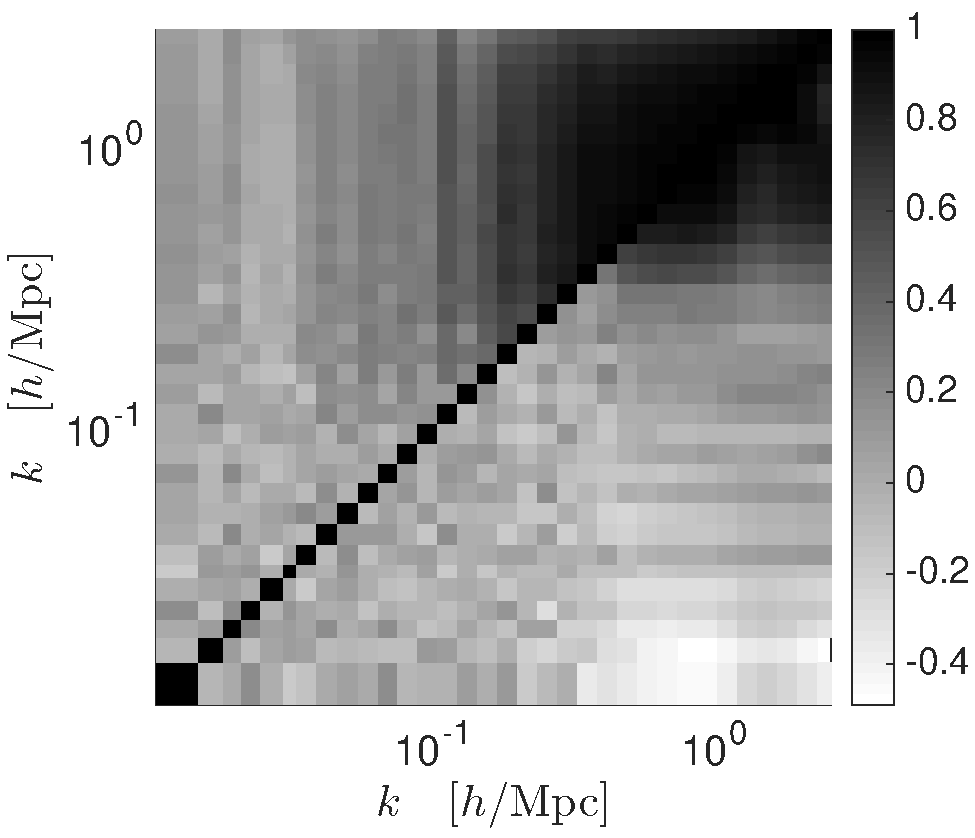
\includegraphics[width=0.48\textwidth]{fig3.pdf}
    \caption{The correlation matrix from 130 non-linear power
      spectra (the upper-left elements) and reconstructed power
      spectra (the lower-right off-diagonal elements).}
    \label{fig:corrall}
  \end{figure}

  The Fisher information is proportional to the volume. 
  We plot the Fisher information per unit volume of the
  simulation, linear and reconstructed power spectra in the left panel of 
  Fig.~\ref{fig:fisherinfo}. The Fisher information of the linear 
  power spectra is equal to the number of $k$ modes within the shell in 
  wave space, $N_k$. We find that the Fisher information of the
  non-linear power spectra drops from the linear one at
  $k \simeq 0.05$ h/Mpc, and has a flat plateau in the non-linear
  regime, with a saturated value of
  $I \simeq 2.5 \times 10^{-5}/\mathrm{(Mpc/h)}^3$.  This indicates
  that there is nearly no independent information in the non-linear
  regime.  However, the information curve of the reconstructed power
  spectra keeps increasing roughly the same as the linear information
  until $k\simeq 0.3$ h/Mpc, and reaches a value of 
  $I \simeq 1.3 \times 10^{-3}/\mathrm{(Mpc/h)}^3$ at $k \simeq 2.6$ h/Mpc, up by a
  factor of 50.  
  This means that the MM reconstructed method can
  strongly recover the lost information within these scales.  
  We compare the Fisher information given by the MM reconstruction method
  with the logarithmic density mapping method \cite{bib:Mark2009} as
  an example to illustrate its strength. We find that MM
  reconstruction gives over 10 times more information than it.  In some papers, the cross correlation $r^2$ terms are set
  to unity in Eq.~\ref{eq:fisherformulaused}, which artificially
  increases the information.  For comparison, we plot this case in the right panel of 
  Fig.~\ref{fig:fisherinfo}.  We see that the logarithmic density
  mapping information is much higher, but only because it is not well
  correlated with the initial conditions.

  Another way to quantify the non-linear scale is via the plateau's linear equivalent scale.  That is, the wavenumber $\kappa$ for which the linear information is the same as the non-linear plateau value, which we take to be at $k \simeq 2.6$ h/Mpc.  We find that the MM reconstruction increases $\kappa$ from $0.15$ to $0.4$ h/Mpc whereas the logarithmic density mapping method only increases it to $0.19$ h/Mpc.

%  Another way to efficiently quantify the information is to give the wavenumber $\kappa$ 
%  where the information of linear power spectra has the same magnitude of 
%  the given information. In the left panel of Fig.~\ref{fig:fisherinfo}, 
%  $\kappa$ is the horizontal coordinates of the intersections of horizonal 
%  dotted lines with the linear information curve. At $k \simeq 2.6$ h/Mpc, MM reconstruction 
%  push $\kappa$ from $0.15$ h/Mpc to $0.4$ h/Mpc, while the logarithmic density mapping method 
%  only pushes $\kappa$ to $0.19$ h/Mpc.

  \begin{figure*}
    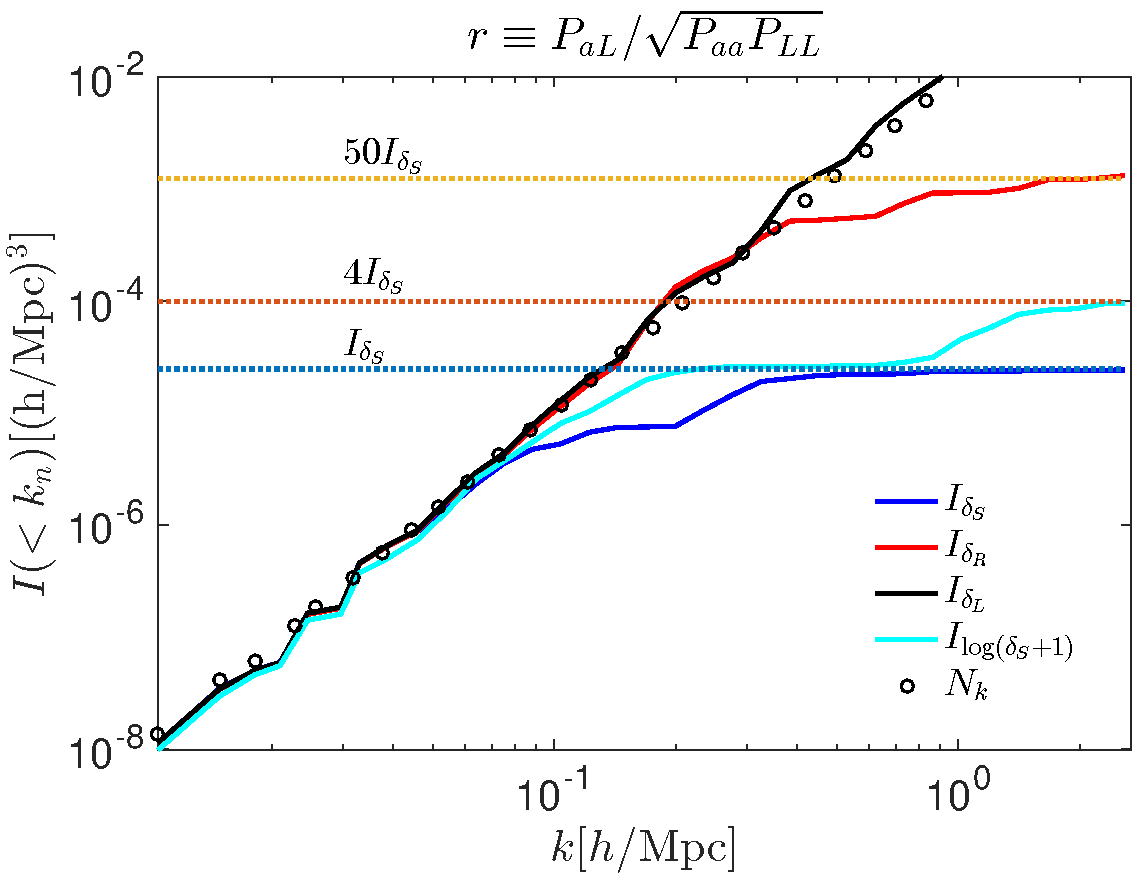
\includegraphics[width=0.48\textwidth]{fig4a.pdf}
    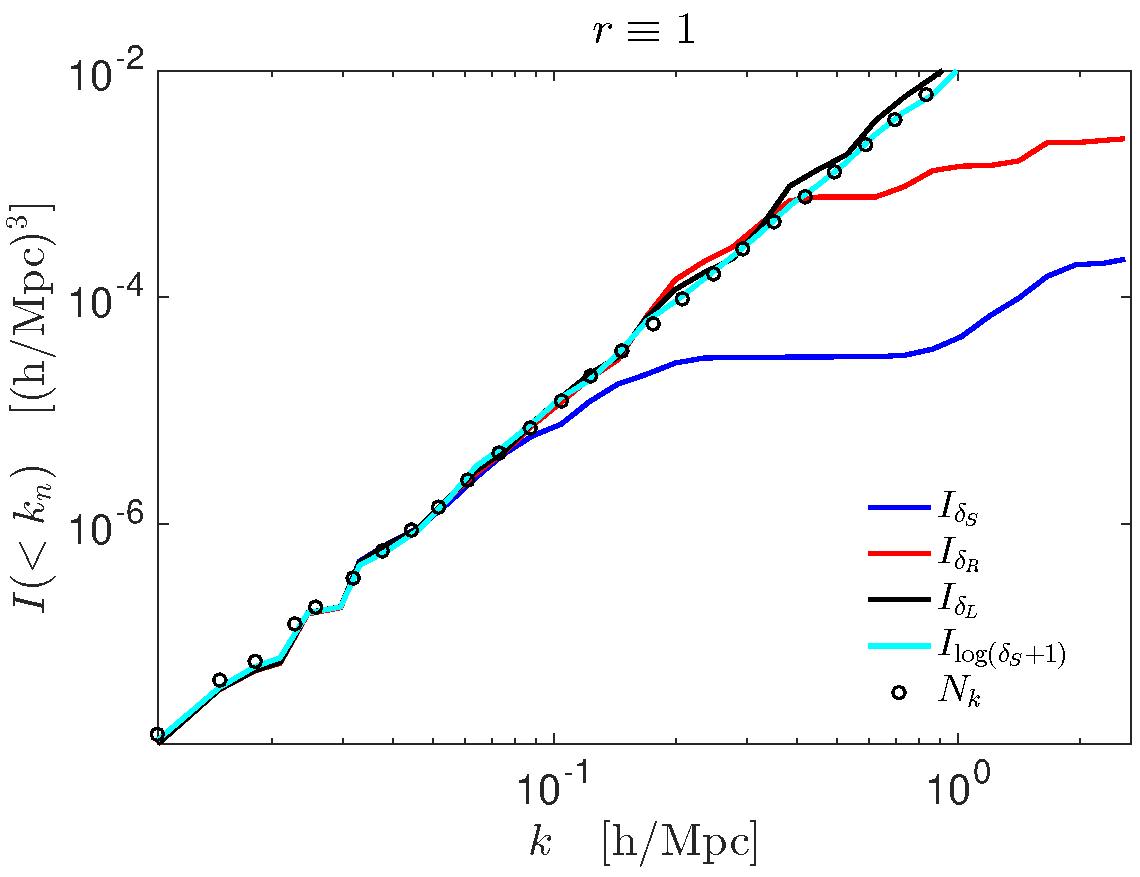
\includegraphics[width=0.48\textwidth]{fig4b.pdf}
    \centering
    \caption{{\it Left.} The Fisher information (solid lines) per unit volume as
      a function of wavenumber.  The blue line corresponds to the
      non-linear density fields, the red line corresponds
      to the the reconstructed density fields, the dark line
      corresponds to the linear density fields, the cyan line
      corresponds to the logarithmic density mapping, and the circles
      are the cumulative number of $k$ modes.  Dotted horizonal lines indicate the value of the 
      Fisher information at $k \simeq 2.6$ h/Mpc.  {\it Right.} Same
      as the left panel except with $r\equiv 1$. The black, blue and cyan lines
      match the results in \cite{bib:Rimes2006,bib:Mark2009}.}
  \label{fig:fisherinfo}
\end{figure*}
\end{section}
